\begin{figure}[htbp]
\centering
\begin{tikzpicture}
\begin{axis}[
    width=\columnwidth,
    height=0.6\textheight,
    xlabel={Age (years)},
    ylabel={Studies},
    grid=major,
    grid style={dashed,gray!30},
    tick style={font=\footnotesize},
    label style={font=\small},
    title style={font=\normalsize},
    title={Age Distribution: Range and Standard Deviation},
    ytick={0,1,2,3,4,5,6,7,8,9,10,11,12,13,14,15,16,17,18,19,20,21,22,23,24,25,26,27,28,29,30,31,32,33,34,35,36,37,38,39,40,41,42,43,44,45,46,47,48,49,50,51,52,53,54,55,56,57,58,59,60,61},
    yticklabels={\cite{liaoUsingEEGDeep2020},\cite{weechInfluenceBoneconductedVibration2018},\cite{huaDetectionVirtualReality2024},\cite{nakataExploringDisplayParameters2025},\cite{zhouApplicationEEGSTransformation2023},\cite{chaiEEGStudyVirtual2023},\cite{qiProfilingCybersicknessBalance2021},\cite{gallagherVectionVirtualReality2019},\cite{liExploringFeasibilityMitigating2020},\cite{shenClassificationVisuallyInduced2024},\cite{dasdemirClassificationEmotionalImmersive2023},\cite{dasdemirLocomotionTechniquesEEG2023},\cite{takeuchiModulationExcitabilityTemporoparietal2018},\cite{lin653QuantizationCybersickness2018},\cite{weechReductionCybersicknessImmediately2020},\cite{huaEEGClassificationModel2024},\cite{linEEGEffectsMotion2007},\cite{liExploringNeuralBiomarkers2023},\cite{chenSpatialTemporalEEG2010},\cite{chenMotionSicknessRelatedBrain2009},\cite{xuAssessingEffectsFullbody2019},\cite{tanimuraEffectsLowResolution3D2019},\cite{fengComprehensiveExplorationMotion2025},\cite{huaAssessmentVirtualReality2023},\cite{huaSiamLSTMModelMultichannel2024},\cite{liMachineLearningAssessment2019},\cite{yangPredictionDetectionVirtual2023},\cite{kimCharacteristicChangesPhysiological2005},\cite{mimnaughVirtualRealitySickness2023},\cite{bergerSexDifferencesUser2021},\cite{tianWhoSaysYou2024},\cite{recentiPredictingMotionSickness2021},\cite{ozkanEffectsSpeedComplexity2023},\cite{changEffectsRestFrames2013},\cite{bergerInfluencePlaceboTDCS2024},\cite{jangEstimatingObjectiveEEG2022},\cite{namElectroencephalogramMicrostatesFunctional2022},\cite{wooRecoveryTimeVR2023},\cite{yeoEEGbasedAnalysisVarious2022},\cite{yeoInvestigatingCorticalActivity2024},\cite{yamamuraHemodynamicVRAdaptingUsers2021},\cite{changIdentifyingPhysiologicalCorrelates2022},\cite{grothOmnidirectionalGalvanicVestibular2022a},\cite{liuExploringQuantitativeAssessment2024},\cite{liuExploringBrainPhysiological2024},\cite{limTestretestReliabilityVirtual2021},\cite{kimPsychophysiologicalAlterationVirtual2019},\cite{khaitamiEEGVisualizationCybersickness2019},\cite{uyanCDMSRealtimeSystem2024},\cite{chiossiMindVisualDiscomfort2024},\cite{cortesEEGbasedExperimentVR2023},\cite{wuInhibitionrelatedN2P32020},\cite{benelliFrequencyDependentReductionCybersickness2023},\cite{andrievskaiaExploringNeurophysiologicalCorrelates2023},\cite{krokosQuantifyingVRCybersickness2022},\cite{abdalhadiDEVELOPMENTVIRTUALENVIRONMENT},\cite{argasinskiElectroencephalographicEEGCorrelates2023},\cite{nurnbergerMismatchVisualVestibularInformation2021},\cite{moinnereauCybersicknessMarkerPrediction2024},\cite{liVRMotionSickness2020},\cite{ahnTemporalDynamicsVisually2020},\cite{pradhanVisualVestibularConflict2022}},
    yticklabel style={font=\tiny},
    xmin=3.5,
    xmax=58.5,
    enlarge y limits=0.05,
    legend pos=south east,
    legend style={font=\tiny},
]

% Mean points
\addplot[only marks, mark=*, mark size=2pt, black] coordinates {
    (16.54, 0)
    (18.63, 1)
    (20.4, 2)
    (20.4, 3)
    (20.4, 4)
    (20.4, 5)
    (21.05, 6)
    (21.13, 7)
    (21.2, 8)
    (21.32, 9)
    (21.44, 10)
    (21.44, 11)
    (21.5, 12)
    (21.96, 13)
    (22.0, 14)
    (22.0, 15)
    (22.0, 16)
    (22.0, 17)
    (22.1, 18)
    (22.1, 19)
    (22.42, 20)
    (22.6, 21)
    (22.8, 22)
    (22.8, 23)
    (22.8, 24)
    (22.8, 25)
    (23.0, 26)
    (23.08, 27)
    (23.11, 28)
    (23.21, 29)
    (23.3, 30)
    (23.8, 31)
    (23.8, 32)
    (23.91, 33)
    (23.95, 34)
    (23.95, 35)
    (24.1, 36)
    (24.1, 37)
    (24.12, 38)
    (24.17, 39)
    (24.2, 40)
    (24.65, 41)
    (24.79, 42)
    (24.8, 43)
    (24.8, 44)
    (25.0, 45)
    (25.0, 46)
    (25.11, 47)
    (25.4, 48)
    (25.4, 49)
    (25.73, 50)
    (25.8, 51)
    (26.3, 52)
    (26.7, 53)
    (27.0, 54)
    (28.0, 55)
    (28.1, 56)
    (28.8, 57)
    (28.9, 58)
    (29.3, 59)
    (29.7, 60)
    (31.0, 61)
};
\addlegendentry{Mean age}

% Age range error bars (min-max)
\draw[black, line width=1.0pt, densely dotted] (axis cs:6.0,0) -- (axis cs:23.0,0);
\draw[black, line width=1.0pt] (axis cs:6.0,-0.15) -- (axis cs:6.0,0.15);
\draw[black, line width=1.0pt] (axis cs:23.0,-0.15) -- (axis cs:23.0,0.15);
\draw[black, line width=1.0pt, densely dotted] (axis cs:17.0,1) -- (axis cs:27.0,1);
\draw[black, line width=1.0pt] (axis cs:17.0,0.85) -- (axis cs:17.0,1.15);
\draw[black, line width=1.0pt] (axis cs:27.0,0.85) -- (axis cs:27.0,1.15);
\draw[black, line width=1.0pt, densely dotted] (axis cs:18.0,10) -- (axis cs:30.0,10);
\draw[black, line width=1.0pt] (axis cs:18.0,9.85) -- (axis cs:18.0,10.15);
\draw[black, line width=1.0pt] (axis cs:30.0,9.85) -- (axis cs:30.0,10.15);
\draw[black, line width=1.0pt, densely dotted] (axis cs:18.0,11) -- (axis cs:30.0,11);
\draw[black, line width=1.0pt] (axis cs:18.0,10.85) -- (axis cs:18.0,11.15);
\draw[black, line width=1.0pt] (axis cs:30.0,10.85) -- (axis cs:30.0,11.15);
\draw[black, line width=1.0pt, densely dotted] (axis cs:20.0,12) -- (axis cs:24.0,12);
\draw[black, line width=1.0pt] (axis cs:20.0,11.85) -- (axis cs:20.0,12.15);
\draw[black, line width=1.0pt] (axis cs:24.0,11.85) -- (axis cs:24.0,12.15);
\draw[black, line width=1.0pt, densely dotted] (axis cs:20.0,13) -- (axis cs:31.0,13);
\draw[black, line width=1.0pt] (axis cs:20.0,12.85) -- (axis cs:20.0,13.15);
\draw[black, line width=1.0pt] (axis cs:31.0,12.85) -- (axis cs:31.0,13.15);
\draw[black, line width=1.0pt, densely dotted] (axis cs:18.0,14) -- (axis cs:56.0,14);
\draw[black, line width=1.0pt] (axis cs:18.0,13.85) -- (axis cs:18.0,14.15);
\draw[black, line width=1.0pt] (axis cs:56.0,13.85) -- (axis cs:56.0,14.15);
\draw[black, line width=1.0pt, densely dotted] (axis cs:19.0,15) -- (axis cs:25.0,15);
\draw[black, line width=1.0pt] (axis cs:19.0,14.85) -- (axis cs:19.0,15.15);
\draw[black, line width=1.0pt] (axis cs:25.0,14.85) -- (axis cs:25.0,15.15);
\draw[black, line width=1.0pt, densely dotted] (axis cs:18.0,16) -- (axis cs:26.0,16);
\draw[black, line width=1.0pt] (axis cs:18.0,15.85) -- (axis cs:18.0,16.15);
\draw[black, line width=1.0pt] (axis cs:26.0,15.85) -- (axis cs:26.0,16.15);
\draw[black, line width=1.0pt, densely dotted] (axis cs:20.0,17) -- (axis cs:32.0,17);
\draw[black, line width=1.0pt] (axis cs:20.0,16.85) -- (axis cs:20.0,17.15);
\draw[black, line width=1.0pt] (axis cs:32.0,16.85) -- (axis cs:32.0,17.15);
\draw[black, line width=1.0pt, densely dotted] (axis cs:21.0,18) -- (axis cs:24.0,18);
\draw[black, line width=1.0pt] (axis cs:21.0,17.85) -- (axis cs:21.0,18.15);
\draw[black, line width=1.0pt] (axis cs:24.0,17.85) -- (axis cs:24.0,18.15);
\draw[black, line width=1.0pt, densely dotted] (axis cs:21.0,19) -- (axis cs:24.0,19);
\draw[black, line width=1.0pt] (axis cs:21.0,18.85) -- (axis cs:21.0,19.15);
\draw[black, line width=1.0pt] (axis cs:24.0,18.85) -- (axis cs:24.0,19.15);
\draw[black, line width=1.0pt, densely dotted] (axis cs:19.0,20) -- (axis cs:29.0,20);
\draw[black, line width=1.0pt] (axis cs:19.0,19.85) -- (axis cs:19.0,20.15);
\draw[black, line width=1.0pt] (axis cs:29.0,19.85) -- (axis cs:29.0,20.15);
\draw[black, line width=1.0pt, densely dotted] (axis cs:18.0,25) -- (axis cs:27.0,25);
\draw[black, line width=1.0pt] (axis cs:18.0,24.85) -- (axis cs:18.0,25.15);
\draw[black, line width=1.0pt] (axis cs:27.0,24.85) -- (axis cs:27.0,25.15);
\draw[black, line width=1.0pt, densely dotted] (axis cs:18.0,26) -- (axis cs:33.0,26);
\draw[black, line width=1.0pt] (axis cs:18.0,25.85) -- (axis cs:18.0,26.15);
\draw[black, line width=1.0pt] (axis cs:33.0,25.85) -- (axis cs:33.0,26.15);
\draw[black, line width=1.0pt, densely dotted] (axis cs:19.0,27) -- (axis cs:27.0,27);
\draw[black, line width=1.0pt] (axis cs:19.0,26.85) -- (axis cs:19.0,27.15);
\draw[black, line width=1.0pt] (axis cs:27.0,26.85) -- (axis cs:27.0,27.15);
\draw[black, line width=1.0pt, densely dotted] (axis cs:18.0,28) -- (axis cs:50.0,28);
\draw[black, line width=1.0pt] (axis cs:18.0,27.85) -- (axis cs:18.0,28.15);
\draw[black, line width=1.0pt] (axis cs:50.0,27.85) -- (axis cs:50.0,28.15);
\draw[black, line width=1.0pt, densely dotted] (axis cs:18.0,29) -- (axis cs:34.0,29);
\draw[black, line width=1.0pt] (axis cs:18.0,28.85) -- (axis cs:18.0,29.15);
\draw[black, line width=1.0pt] (axis cs:34.0,28.85) -- (axis cs:34.0,29.15);
\draw[black, line width=1.0pt, densely dotted] (axis cs:20.0,30) -- (axis cs:45.0,30);
\draw[black, line width=1.0pt] (axis cs:20.0,29.85) -- (axis cs:20.0,30.15);
\draw[black, line width=1.0pt] (axis cs:45.0,29.85) -- (axis cs:45.0,30.15);
\draw[black, line width=1.0pt, densely dotted] (axis cs:18.0,32) -- (axis cs:42.0,32);
\draw[black, line width=1.0pt] (axis cs:18.0,31.85) -- (axis cs:18.0,32.15);
\draw[black, line width=1.0pt] (axis cs:42.0,31.85) -- (axis cs:42.0,32.15);
\draw[black, line width=1.0pt, densely dotted] (axis cs:18.0,34) -- (axis cs:34.0,34);
\draw[black, line width=1.0pt] (axis cs:18.0,33.85) -- (axis cs:18.0,34.15);
\draw[black, line width=1.0pt] (axis cs:34.0,33.85) -- (axis cs:34.0,34.15);
\draw[black, line width=1.0pt, densely dotted] (axis cs:19.0,42) -- (axis cs:52.0,42);
\draw[black, line width=1.0pt] (axis cs:19.0,41.85) -- (axis cs:19.0,42.15);
\draw[black, line width=1.0pt] (axis cs:52.0,41.85) -- (axis cs:52.0,42.15);
\draw[black, line width=1.0pt, densely dotted] (axis cs:20.0,46) -- (axis cs:37.0,46);
\draw[black, line width=1.0pt] (axis cs:20.0,45.85) -- (axis cs:20.0,46.15);
\draw[black, line width=1.0pt] (axis cs:37.0,45.85) -- (axis cs:37.0,46.15);
\draw[black, line width=1.0pt, densely dotted] (axis cs:19.0,47) -- (axis cs:30.0,47);
\draw[black, line width=1.0pt] (axis cs:19.0,46.85) -- (axis cs:19.0,47.15);
\draw[black, line width=1.0pt] (axis cs:30.0,46.85) -- (axis cs:30.0,47.15);
\draw[black, line width=1.0pt, densely dotted] (axis cs:18.0,48) -- (axis cs:42.0,48);
\draw[black, line width=1.0pt] (axis cs:18.0,47.85) -- (axis cs:18.0,48.15);
\draw[black, line width=1.0pt] (axis cs:42.0,47.85) -- (axis cs:42.0,48.15);
\draw[black, line width=1.0pt, densely dotted] (axis cs:19.0,53) -- (axis cs:44.0,53);
\draw[black, line width=1.0pt] (axis cs:19.0,52.85) -- (axis cs:19.0,53.15);
\draw[black, line width=1.0pt] (axis cs:44.0,52.85) -- (axis cs:44.0,53.15);
\draw[black, line width=1.0pt, densely dotted] (axis cs:18.0,56) -- (axis cs:42.0,56);
\draw[black, line width=1.0pt] (axis cs:18.0,55.85) -- (axis cs:18.0,56.15);
\draw[black, line width=1.0pt] (axis cs:42.0,55.85) -- (axis cs:42.0,56.15);
\draw[black, line width=1.0pt, densely dotted] (axis cs:23.0,57) -- (axis cs:37.0,57);
\draw[black, line width=1.0pt] (axis cs:23.0,56.85) -- (axis cs:23.0,57.15);
\draw[black, line width=1.0pt] (axis cs:37.0,56.85) -- (axis cs:37.0,57.15);
\draw[black, line width=1.0pt, densely dotted] (axis cs:21.0,60) -- (axis cs:48.0,60);
\draw[black, line width=1.0pt] (axis cs:21.0,59.85) -- (axis cs:21.0,60.15);
\draw[black, line width=1.0pt] (axis cs:48.0,59.85) -- (axis cs:48.0,60.15);

% Standard deviation error bars (mean ± std)
\draw[gray, line width=1.0pt] (axis cs:14.37,0) -- (axis cs:18.71,0);
\draw[gray, line width=1.0pt] (axis cs:14.37,-0.1) -- (axis cs:14.37,0.1);
\draw[gray, line width=1.0pt] (axis cs:18.71,-0.1) -- (axis cs:18.71,0.1);
\draw[gray, line width=1.0pt] (axis cs:17.11,1) -- (axis cs:20.15,1);
\draw[gray, line width=1.0pt] (axis cs:17.11,0.9) -- (axis cs:17.11,1.1);
\draw[gray, line width=1.0pt] (axis cs:20.15,0.9) -- (axis cs:20.15,1.1);
\draw[gray, line width=1.0pt] (axis cs:18.9,2) -- (axis cs:21.9,2);
\draw[gray, line width=1.0pt] (axis cs:18.9,1.9) -- (axis cs:18.9,2.1);
\draw[gray, line width=1.0pt] (axis cs:21.9,1.9) -- (axis cs:21.9,2.1);
\draw[gray, line width=1.0pt] (axis cs:18.4,3) -- (axis cs:22.4,3);
\draw[gray, line width=1.0pt] (axis cs:18.4,2.9) -- (axis cs:18.4,3.1);
\draw[gray, line width=1.0pt] (axis cs:22.4,2.9) -- (axis cs:22.4,3.1);
\draw[gray, line width=1.0pt] (axis cs:18.9,4) -- (axis cs:21.9,4);
\draw[gray, line width=1.0pt] (axis cs:18.9,3.9) -- (axis cs:18.9,4.1);
\draw[gray, line width=1.0pt] (axis cs:21.9,3.9) -- (axis cs:21.9,4.1);
\draw[gray, line width=1.0pt] (axis cs:18.9,5) -- (axis cs:21.9,5);
\draw[gray, line width=1.0pt] (axis cs:18.9,4.9) -- (axis cs:18.9,5.1);
\draw[gray, line width=1.0pt] (axis cs:21.9,4.9) -- (axis cs:21.9,5.1);
\draw[gray, line width=1.0pt] (axis cs:19.080000000000002,6) -- (axis cs:23.02,6);
\draw[gray, line width=1.0pt] (axis cs:19.080000000000002,5.9) -- (axis cs:19.080000000000002,6.1);
\draw[gray, line width=1.0pt] (axis cs:23.02,5.9) -- (axis cs:23.02,6.1);
\draw[gray, line width=1.0pt] (axis cs:17.23,7) -- (axis cs:25.029999999999998,7);
\draw[gray, line width=1.0pt] (axis cs:17.23,6.9) -- (axis cs:17.23,7.1);
\draw[gray, line width=1.0pt] (axis cs:25.029999999999998,6.9) -- (axis cs:25.029999999999998,7.1);
\draw[gray, line width=1.0pt] (axis cs:19.05,9) -- (axis cs:23.59,9);
\draw[gray, line width=1.0pt] (axis cs:19.05,8.9) -- (axis cs:19.05,9.1);
\draw[gray, line width=1.0pt] (axis cs:23.59,8.9) -- (axis cs:23.59,9.1);
\draw[gray, line width=1.0pt] (axis cs:19.32,10) -- (axis cs:23.560000000000002,10);
\draw[gray, line width=1.0pt] (axis cs:19.32,9.9) -- (axis cs:19.32,10.1);
\draw[gray, line width=1.0pt] (axis cs:23.560000000000002,9.9) -- (axis cs:23.560000000000002,10.1);
\draw[gray, line width=1.0pt] (axis cs:19.32,11) -- (axis cs:23.560000000000002,11);
\draw[gray, line width=1.0pt] (axis cs:19.32,10.9) -- (axis cs:19.32,11.1);
\draw[gray, line width=1.0pt] (axis cs:23.560000000000002,10.9) -- (axis cs:23.560000000000002,11.1);
\draw[gray, line width=1.0pt] (axis cs:20.4,12) -- (axis cs:22.6,12);
\draw[gray, line width=1.0pt] (axis cs:20.4,11.9) -- (axis cs:20.4,12.1);
\draw[gray, line width=1.0pt] (axis cs:22.6,11.9) -- (axis cs:22.6,12.1);
\draw[gray, line width=1.0pt] (axis cs:19.69,13) -- (axis cs:24.23,13);
\draw[gray, line width=1.0pt] (axis cs:19.69,12.9) -- (axis cs:19.69,13.1);
\draw[gray, line width=1.0pt] (axis cs:24.23,12.9) -- (axis cs:24.23,13.1);
\draw[gray, line width=1.0pt] (axis cs:14.96,14) -- (axis cs:29.04,14);
\draw[gray, line width=1.0pt] (axis cs:14.96,13.9) -- (axis cs:14.96,14.1);
\draw[gray, line width=1.0pt] (axis cs:29.04,13.9) -- (axis cs:29.04,14.1);
\draw[gray, line width=1.0pt] (axis cs:21.6,21) -- (axis cs:23.6,21);
\draw[gray, line width=1.0pt] (axis cs:21.6,20.9) -- (axis cs:21.6,21.1);
\draw[gray, line width=1.0pt] (axis cs:23.6,20.9) -- (axis cs:23.6,21.1);
\draw[gray, line width=1.0pt] (axis cs:21.7,22) -- (axis cs:23.900000000000002,22);
\draw[gray, line width=1.0pt] (axis cs:21.7,21.9) -- (axis cs:21.7,22.1);
\draw[gray, line width=1.0pt] (axis cs:23.900000000000002,21.9) -- (axis cs:23.900000000000002,22.1);
\draw[gray, line width=1.0pt] (axis cs:21.7,23) -- (axis cs:23.900000000000002,23);
\draw[gray, line width=1.0pt] (axis cs:21.7,22.9) -- (axis cs:21.7,23.1);
\draw[gray, line width=1.0pt] (axis cs:23.900000000000002,22.9) -- (axis cs:23.900000000000002,23.1);
\draw[gray, line width=1.0pt] (axis cs:21.7,24) -- (axis cs:23.900000000000002,24);
\draw[gray, line width=1.0pt] (axis cs:21.7,23.9) -- (axis cs:21.7,24.1);
\draw[gray, line width=1.0pt] (axis cs:23.900000000000002,23.9) -- (axis cs:23.900000000000002,24.1);
\draw[gray, line width=1.0pt] (axis cs:18.9,26) -- (axis cs:27.1,26);
\draw[gray, line width=1.0pt] (axis cs:18.9,25.9) -- (axis cs:18.9,26.1);
\draw[gray, line width=1.0pt] (axis cs:27.1,25.9) -- (axis cs:27.1,26.1);
\draw[gray, line width=1.0pt] (axis cs:21.029999999999998,27) -- (axis cs:25.13,27);
\draw[gray, line width=1.0pt] (axis cs:21.029999999999998,26.9) -- (axis cs:21.029999999999998,27.1);
\draw[gray, line width=1.0pt] (axis cs:25.13,26.9) -- (axis cs:25.13,27.1);
\draw[gray, line width=1.0pt] (axis cs:16.24,28) -- (axis cs:29.98,28);
\draw[gray, line width=1.0pt] (axis cs:16.24,27.9) -- (axis cs:16.24,28.1);
\draw[gray, line width=1.0pt] (axis cs:29.98,27.9) -- (axis cs:29.98,28.1);
\draw[gray, line width=1.0pt] (axis cs:19.8,29) -- (axis cs:26.62,29);
\draw[gray, line width=1.0pt] (axis cs:19.8,28.9) -- (axis cs:19.8,29.1);
\draw[gray, line width=1.0pt] (axis cs:26.62,28.9) -- (axis cs:26.62,29.1);
\draw[gray, line width=1.0pt] (axis cs:18.9,30) -- (axis cs:27.700000000000003,30);
\draw[gray, line width=1.0pt] (axis cs:18.9,29.9) -- (axis cs:18.9,30.1);
\draw[gray, line width=1.0pt] (axis cs:27.700000000000003,29.9) -- (axis cs:27.700000000000003,30.1);
\draw[gray, line width=1.0pt] (axis cs:22.6,31) -- (axis cs:25.0,31);
\draw[gray, line width=1.0pt] (axis cs:22.6,30.9) -- (axis cs:22.6,31.1);
\draw[gray, line width=1.0pt] (axis cs:25.0,30.9) -- (axis cs:25.0,31.1);
\draw[gray, line width=1.0pt] (axis cs:18.240000000000002,32) -- (axis cs:29.36,32);
\draw[gray, line width=1.0pt] (axis cs:18.240000000000002,31.9) -- (axis cs:18.240000000000002,32.1);
\draw[gray, line width=1.0pt] (axis cs:29.36,31.9) -- (axis cs:29.36,32.1);
\draw[gray, line width=1.0pt] (axis cs:22.03,33) -- (axis cs:25.79,33);
\draw[gray, line width=1.0pt] (axis cs:22.03,32.9) -- (axis cs:22.03,33.1);
\draw[gray, line width=1.0pt] (axis cs:25.79,32.9) -- (axis cs:25.79,33.1);
\draw[gray, line width=1.0pt] (axis cs:21.99,35) -- (axis cs:25.91,35);
\draw[gray, line width=1.0pt] (axis cs:21.99,34.9) -- (axis cs:21.99,35.1);
\draw[gray, line width=1.0pt] (axis cs:25.91,34.9) -- (axis cs:25.91,35.1);
\draw[gray, line width=1.0pt] (axis cs:21.8,36) -- (axis cs:26.400000000000002,36);
\draw[gray, line width=1.0pt] (axis cs:21.8,35.9) -- (axis cs:21.8,36.1);
\draw[gray, line width=1.0pt] (axis cs:26.400000000000002,35.9) -- (axis cs:26.400000000000002,36.1);
\draw[gray, line width=1.0pt] (axis cs:21.8,37) -- (axis cs:26.400000000000002,37);
\draw[gray, line width=1.0pt] (axis cs:21.8,36.9) -- (axis cs:21.8,37.1);
\draw[gray, line width=1.0pt] (axis cs:26.400000000000002,36.9) -- (axis cs:26.400000000000002,37.1);
\draw[gray, line width=1.0pt] (axis cs:21.32,38) -- (axis cs:26.92,38);
\draw[gray, line width=1.0pt] (axis cs:21.32,37.9) -- (axis cs:21.32,38.1);
\draw[gray, line width=1.0pt] (axis cs:26.92,37.9) -- (axis cs:26.92,38.1);
\draw[gray, line width=1.0pt] (axis cs:20.8,39) -- (axis cs:27.540000000000003,39);
\draw[gray, line width=1.0pt] (axis cs:20.8,38.9) -- (axis cs:20.8,39.1);
\draw[gray, line width=1.0pt] (axis cs:27.540000000000003,38.9) -- (axis cs:27.540000000000003,39.1);
\draw[gray, line width=1.0pt] (axis cs:22.869999999999997,40) -- (axis cs:25.53,40);
\draw[gray, line width=1.0pt] (axis cs:22.869999999999997,39.9) -- (axis cs:22.869999999999997,40.1);
\draw[gray, line width=1.0pt] (axis cs:25.53,39.9) -- (axis cs:25.53,40.1);
\draw[gray, line width=1.0pt] (axis cs:22.169999999999998,41) -- (axis cs:27.13,41);
\draw[gray, line width=1.0pt] (axis cs:22.169999999999998,40.9) -- (axis cs:22.169999999999998,41.1);
\draw[gray, line width=1.0pt] (axis cs:27.13,40.9) -- (axis cs:27.13,41.1);
\draw[gray, line width=1.0pt] (axis cs:19.07,42) -- (axis cs:30.509999999999998,42);
\draw[gray, line width=1.0pt] (axis cs:19.07,41.9) -- (axis cs:19.07,42.1);
\draw[gray, line width=1.0pt] (axis cs:30.509999999999998,41.9) -- (axis cs:30.509999999999998,42.1);
\draw[gray, line width=1.0pt] (axis cs:21.2,43) -- (axis cs:28.400000000000002,43);
\draw[gray, line width=1.0pt] (axis cs:21.2,42.9) -- (axis cs:21.2,43.1);
\draw[gray, line width=1.0pt] (axis cs:28.400000000000002,42.9) -- (axis cs:28.400000000000002,43.1);
\draw[gray, line width=1.0pt] (axis cs:21.2,44) -- (axis cs:28.400000000000002,44);
\draw[gray, line width=1.0pt] (axis cs:21.2,43.9) -- (axis cs:21.2,44.1);
\draw[gray, line width=1.0pt] (axis cs:28.400000000000002,43.9) -- (axis cs:28.400000000000002,44.1);
\draw[gray, line width=1.0pt] (axis cs:22.8,45) -- (axis cs:27.2,45);
\draw[gray, line width=1.0pt] (axis cs:22.8,44.9) -- (axis cs:22.8,45.1);
\draw[gray, line width=1.0pt] (axis cs:27.2,44.9) -- (axis cs:27.2,45.1);
\draw[gray, line width=1.0pt] (axis cs:21.0,46) -- (axis cs:29.0,46);
\draw[gray, line width=1.0pt] (axis cs:21.0,45.9) -- (axis cs:21.0,46.1);
\draw[gray, line width=1.0pt] (axis cs:29.0,45.9) -- (axis cs:29.0,46.1);
\draw[gray, line width=1.0pt] (axis cs:20.599999999999998,49) -- (axis cs:30.2,49);
\draw[gray, line width=1.0pt] (axis cs:20.599999999999998,48.9) -- (axis cs:20.599999999999998,49.1);
\draw[gray, line width=1.0pt] (axis cs:30.2,48.9) -- (axis cs:30.2,49.1);
\draw[gray, line width=1.0pt] (axis cs:22.13,50) -- (axis cs:29.330000000000002,50);
\draw[gray, line width=1.0pt] (axis cs:22.13,49.9) -- (axis cs:22.13,50.1);
\draw[gray, line width=1.0pt] (axis cs:29.330000000000002,49.9) -- (axis cs:29.330000000000002,50.1);
\draw[gray, line width=1.0pt] (axis cs:23.900000000000002,51) -- (axis cs:27.7,51);
\draw[gray, line width=1.0pt] (axis cs:23.900000000000002,50.9) -- (axis cs:23.900000000000002,51.1);
\draw[gray, line width=1.0pt] (axis cs:27.7,50.9) -- (axis cs:27.7,51.1);
\draw[gray, line width=1.0pt] (axis cs:23.5,52) -- (axis cs:29.1,52);
\draw[gray, line width=1.0pt] (axis cs:23.5,51.9) -- (axis cs:23.5,52.1);
\draw[gray, line width=1.0pt] (axis cs:29.1,51.9) -- (axis cs:29.1,52.1);
\draw[gray, line width=1.0pt] (axis cs:20.38,53) -- (axis cs:33.019999999999996,53);
\draw[gray, line width=1.0pt] (axis cs:20.38,52.9) -- (axis cs:20.38,53.1);
\draw[gray, line width=1.0pt] (axis cs:33.019999999999996,52.9) -- (axis cs:33.019999999999996,53.1);
\draw[gray, line width=1.0pt] (axis cs:19.0,54) -- (axis cs:35.0,54);
\draw[gray, line width=1.0pt] (axis cs:19.0,53.9) -- (axis cs:19.0,54.1);
\draw[gray, line width=1.0pt] (axis cs:35.0,53.9) -- (axis cs:35.0,54.1);
\draw[gray, line width=1.0pt] (axis cs:26.0,55) -- (axis cs:30.0,55);
\draw[gray, line width=1.0pt] (axis cs:26.0,54.9) -- (axis cs:26.0,55.1);
\draw[gray, line width=1.0pt] (axis cs:30.0,54.9) -- (axis cs:30.0,55.1);
\draw[gray, line width=1.0pt] (axis cs:22.490000000000002,56) -- (axis cs:33.71,56);
\draw[gray, line width=1.0pt] (axis cs:22.490000000000002,55.9) -- (axis cs:22.490000000000002,56.1);
\draw[gray, line width=1.0pt] (axis cs:33.71,55.9) -- (axis cs:33.71,56.1);
\draw[gray, line width=1.0pt] (axis cs:25.400000000000002,57) -- (axis cs:32.2,57);
\draw[gray, line width=1.0pt] (axis cs:25.400000000000002,56.9) -- (axis cs:25.400000000000002,57.1);
\draw[gray, line width=1.0pt] (axis cs:32.2,56.9) -- (axis cs:32.2,57.1);
\draw[gray, line width=1.0pt] (axis cs:26.0,58) -- (axis cs:31.799999999999997,58);
\draw[gray, line width=1.0pt] (axis cs:26.0,57.9) -- (axis cs:26.0,58.1);
\draw[gray, line width=1.0pt] (axis cs:31.799999999999997,57.9) -- (axis cs:31.799999999999997,58.1);
\draw[gray, line width=1.0pt] (axis cs:22.0,61) -- (axis cs:40.0,61);
\draw[gray, line width=1.0pt] (axis cs:22.0,60.9) -- (axis cs:22.0,61.1);
\draw[gray, line width=1.0pt] (axis cs:40.0,60.9) -- (axis cs:40.0,61.1);

% Legend entries
\addlegendimage{gray, line width=1.0pt}
\addlegendentry{Standard deviation}
\addlegendimage{black, line width=1.0pt, densely dotted}
\addlegendentry{Min/Max range}

\end{axis}
\end{tikzpicture}
\caption{Age distribution across studies showing mean age (black dots) with age ranges (dotted bars) and standard deviations when available (solid bars). The age range shows the minimum and maximum participant ages, while the standard deviation shows the typical spread around the mean age.}
\label{fig:age_distribution}
\end{figure}
